\subsection{Diagram Klas}

Przedstawiony na poniższym obrazku diagram klas reprezentuje wszystkie
wykorzystywane przez Zleceniodawcę elementy składające się na cały system.
Diagram ten ma znaczenie przede wszystkim dla deweloperów i osób zajmujących się
wytwarzaniem oprogramowania, tym niemniej powinien zostać zatwierdzony przed
przedstawicieli Zleceniodawcy - diagram klas jest bowiem punktem łączącym z
jednej strony wyobrażenie klienta o podziale funkcjonalności a z drugiej decyzje
projektowe podjęte przez zespół zajmujący się implementacją.

Diagram klas powinien obrazować zależności (agregacje, kompozycje, relację
dziedziczenia) pomiędzy poszczególnymi klasami na tyle szczegółowo, by osoby 
nieposiadające wykształcenia informatycznego i nieznające metod programowania
obiektowego mogłby zrozumieć zasadę podziału bez szczegółowych wyjaśnień. Z tego
też powodu na poniższym rysunku skoncentrowano się na powiązaniach pomiędzy
poszczególnymi klasami a nie na nazywaniu i przedstawianiu atrybutów i metod
poszczególnych klas. Nie stanowią one żadnej wartości z punktu widzenia
Zleceniodawcy a mogą stanowić ograniczenie i usztywnienie schematu dla
deweloperów, którzy lepiej znają metody dostarczania funkcjonalności i będą
mogli lepiej modyfikować schemat w zależności od potrzeb, nie naruszając
jednocześnie warunków umowy. Wszystkie atrybuty czy operacje ważne z punktu
widzenia Zleceniodawcy, które mogą mieć wpływ na ocenę projektu zostały
umieszczone na diagramie.

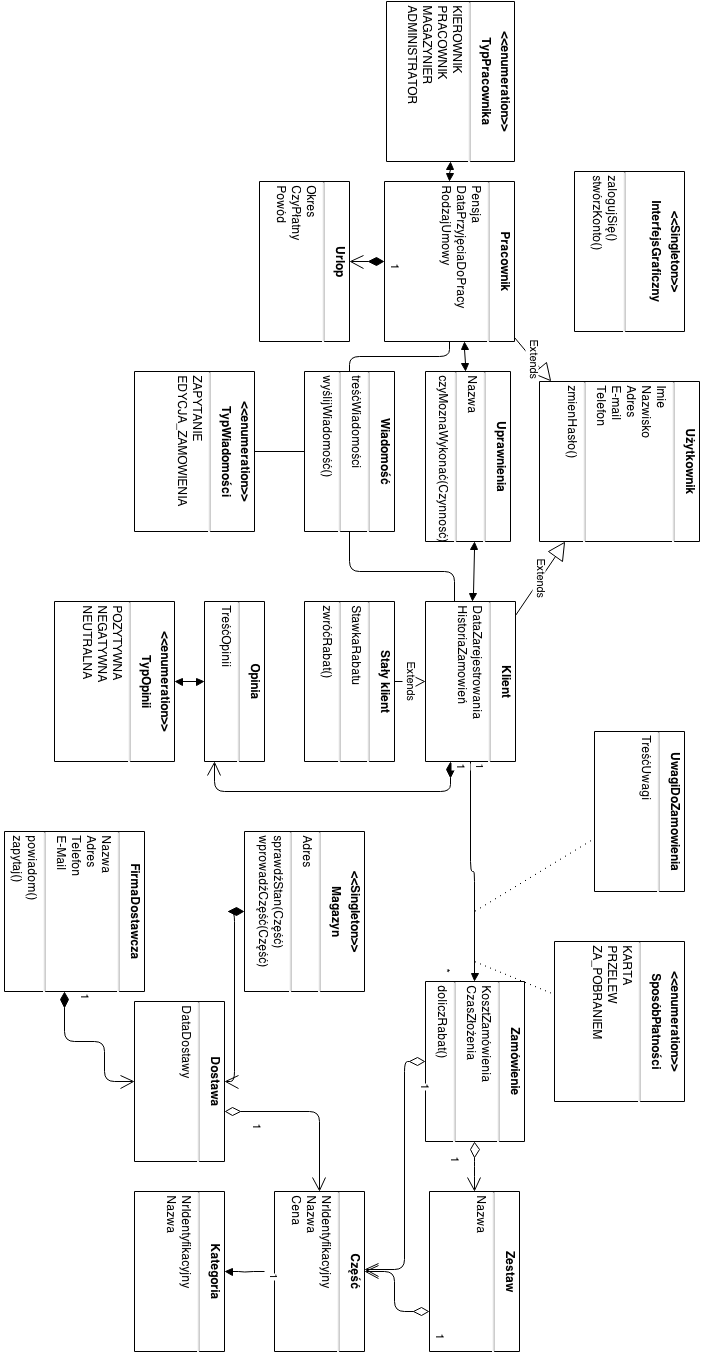
\includegraphics[width=\textwidth,
height=0.8\textheight]{graphics/ClassDiagram.png}
